\documentclass[handout]{beamer}

\usepackage{Haust2017glærur}

\title{Stærðfræðimynstur í tölvunarfræði}
\subtitle{Vika 12, fyrri fyrirlestur}

\begin{document}

\begin{frame}
\titlepage
\end{frame}


\section{Inngangur}

\begin{frame}{Í síðasta tíma}
\begin{itemize}
 \item Hamilton-vegir
 \item Leit að stystu vegum
 \item Farandssöluvandamálið
\end{itemize}
\end{frame}

\section{Lagnet}

\begin{frame}{Lagnet}
\begin{tcolorbox}[title=Lagnet]
Net er kallað lagnet (e. \emph{planar graph}) sé hægt að teikna það í sléttan flöt þannig að hnútar séu punktar og leggirnir samfelldir einfaldir ferlar sem skerast aldrei nema í endapunktunum. Slík teikning er kölluð sléttunet (e. \emph{planar representation}).
\end{tcolorbox}
\end{frame}

\begin{frame}{Dæmi}
\begin{center}
Netið $K_4$ er lagnet. \pause

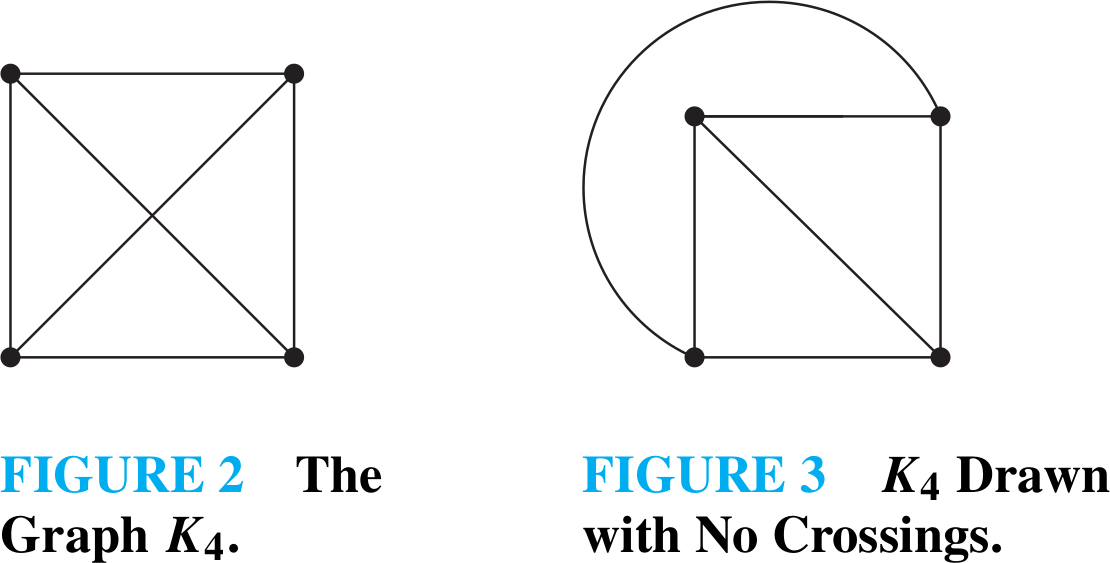
\includegraphics[width=0.8\textwidth]{graph-planar-k4}
\end{center}
\end{frame}

\begin{frame}{Setning Fárys}
    \begin{tcolorbox}[title=Setning Fárys]
        Sérhvert einfalt lagnet á sér sléttunet þar sem leggirnir eru táknaðir með línustrikum.
    \end{tcolorbox}
\end{frame}

\begin{frame}{Dæmi}
\begin{center}
Netið $Q_3$ er lagnet.

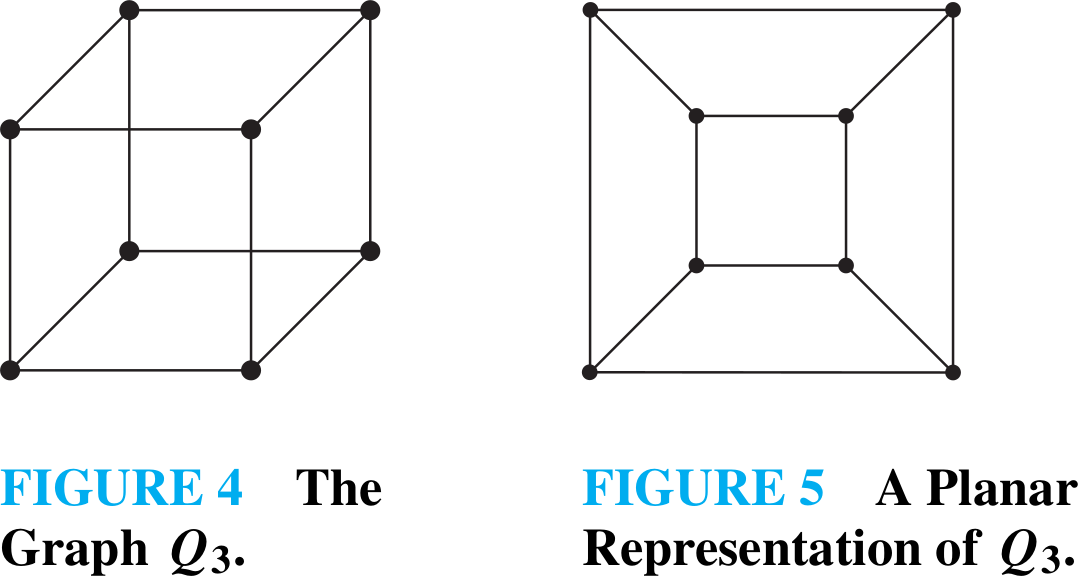
\includegraphics[width=0.8\textwidth]{graph-planar-q3}
\end{center}
\end{frame}

\begin{frame}{Dæmi}
\begin{center}
Netið $K_{3,3}$ er ekki lagnet.

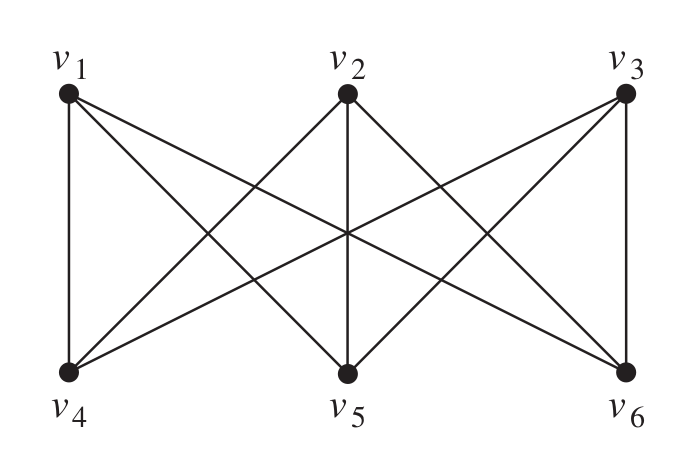
\includegraphics[width=0.8\textwidth]{graph-nonplanar-k33}
\end{center}
\end{frame}

\section{Möskvar}

\begin{frame}{Möskvar}
\begin{columns}
\column{0.5\textwidth}
Sléttuneti má skipta upp í svæði sem kallast möskvar (e. \emph{regions}). Einn möskvinn er ótakmarkað svæði, hinir afmarkast af leggjum netsins.
\column{0.5\textwidth}
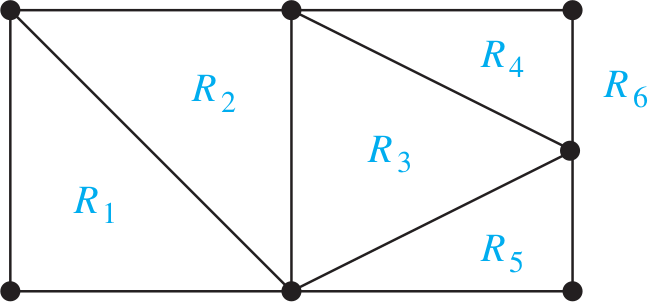
\includegraphics[width=\linewidth]{graph-regions}

Hér eru möskvar netsins merktir með $R_i$.
\end{columns}
\end{frame}

\begin{frame}{Jafna}
\begin{tcolorbox}[title=Jafna Eulers]
Látum $G$ vera einfalt samanhangandi lagnet með $e$ leggjum, $v$ hnútum og $r$ möskvum. Þá er

\[
 r = e - v + 2.
\]

\end{tcolorbox}
\end{frame}

\begin{frame}{Dæmi}
    Hversu marga möskva hefur sléttunetið $Q_3$?

    \pause

    Höfum 8 hnúta og 12 leggi. Þá er 
    \begin{align*}
        r &= e - v + 2\\
          &= 12 - 8 + 2\\
          &= 6
    \end{align*}
    sem við bjuggumst við, því netið er ``teningslaga''.
\end{frame}

\begin{frame}{Dæmi}
Hversu marga möskva hefur sléttunet með 20 hnútum sem allir eru af stigi 3?
\pause

\vspace{1cm}
Hér er $v=20$. Summa stiganna er $3v = 60$. Handabandssetning gefur að summan sé $2e$, svo $e = 30$. Þá gefur jafna Eulers:

\[
 r = e - v + 2 = 30 - 20 + 2 = 12
\]

\end{frame}

\begin{frame}{Fylgisetningar}
Eftirfarandi fylgisetningar eiga við einfalt samanhangandi lagnet $G$ með $v$ hnúta og $e$ leggi:
\begin{tcolorbox}
Sé $v \geq 3$, þá er $e \leq 3v - 6$.
\end{tcolorbox}

\begin{tcolorbox}
$G$ hefur hnút af stigi sem er ekki hærra en $5$.
\end{tcolorbox}

\begin{tcolorbox}
Hafi $G$ engar rásir af lengd 3 og $v \geq 3$, þá er $e \leq 2v -4$
\end{tcolorbox}
Getum notað síðustu fylgisetninguna til að sýna að $K_{3,3}$ sé ekki lagnet.
\end{frame}

\begin{frame}{Maximum planar graph}
    \begin{columns}
        \column{0.4\textwidth}
        \begin{itemize}
            \item Einfalt lagnet er ``maximal planar'' sé ekki hægt að bæta við það legg án þess að 
            \item Sjá einnig: Að skipta á svæði niður í þríhyrninga, mikilvægt í tölvugrafík
        \end{itemize}
        \column{0.6\textwidth}
        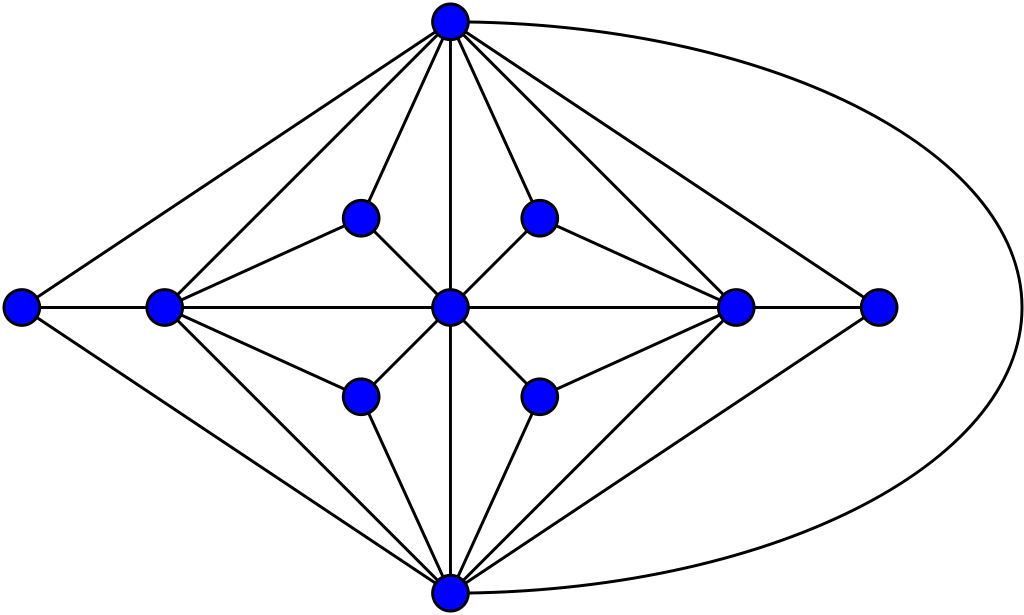
\includegraphics[width=\linewidth]{goldner-harary}
        \begin{center}
            Mynd: \href{https://en.wikipedia.org/wiki/File:Goldner-Harary\_graph.svg}{Wikipedia}
        \end{center}
    \end{columns}
\end{frame}

\begin{frame}{Setning Kuratowskis}
\begin{tcolorbox}[title=Setning Kuratowskis]
Net $G$ er lagnet þá og því aðeins að það innihaldi ekkert hlutnet sem er grannmóta $K_5$ eða $K_{3,3}$.
\end{tcolorbox}
\end{frame}

\section{Hnútalitun}

\begin{frame}{Hnútalitun}
\begin{tcolorbox}[title=Litun]
Litun (e. \emph{coloring}) á einföldu neti er ákvörðun á litum á hverjum hnút netsins svo að engir tveir aðlægir hnútar hafi sama lit.
\end{tcolorbox}

\begin{tcolorbox}[title=Litunartala]
Litunartala nets $G$ er minnsti fjöldi lita sem þarf til að lita hnúta netsins. Litunartala $G$ er táknuð með $\chi(G)$.
\end{tcolorbox}

\end{frame}

\begin{frame}{Fjögurra lita setningin}
\begin{tcolorbox}[title=Fjögurra lita setningin]
Litunartala lagnets er ekki hærri en 4.
\end{tcolorbox}
Setningin var upphaflega sett fram sem tilgáta um miðja 19. öld. Hún var sönnuð árið 1976, þá með aðstoð tölvu.
\end{frame}

\begin{frame}{4 lita heimskort}
    \begin{center}
        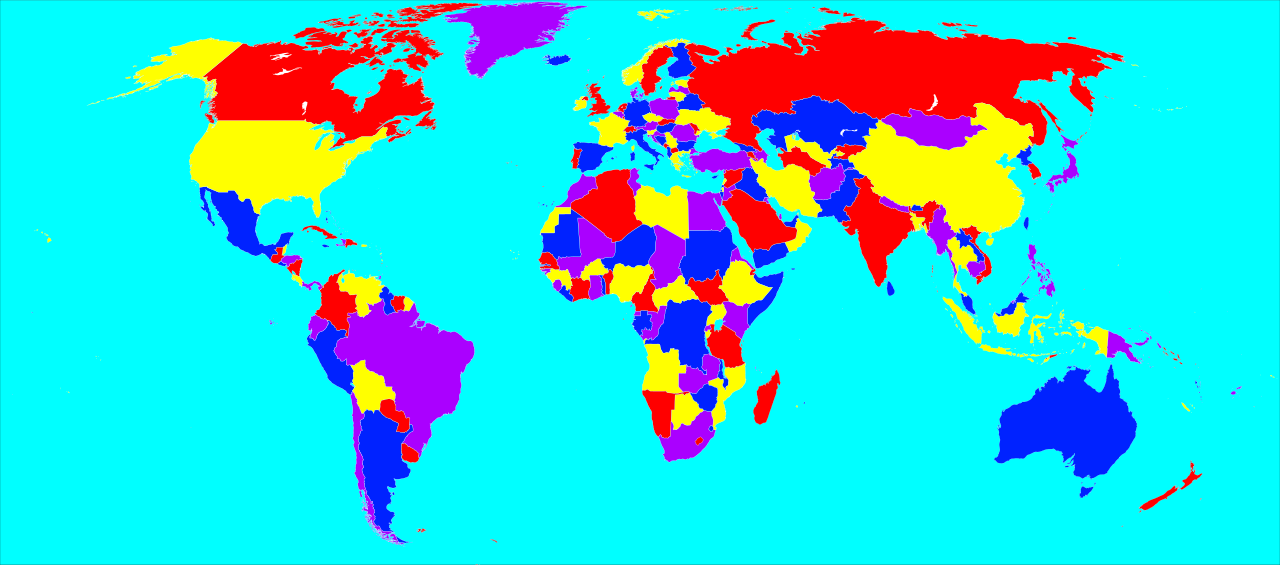
\includegraphics[width=\textwidth]{4colors}
    
    Mynd: \href{https://commons.wikimedia.org/wiki/File:World_map_with_four_colours.svg}{Wikipedia}
    \end{center}
\end{frame}

\begin{frame}{Hagnýtingar}
\begin{itemize}
 \item Hnútalitanir má hagnýta á ýmsa vegu
 \begin{itemize}
  \item Litum landakort
  \begin{itemize}
   \item Lönd eru hnútar, landamæri eru leggir
  \end{itemize}
  \item Ákvörðum tímasetningar fyrir lokapróf (sjá: scheduling problems)
  \begin{itemize}
   \item Táknum námskeið með hnútum, leggur á milli séu námskeiðin tekin af sömu nemendum
   \item Hver möguleg tímasetning fyrir próf er einn litur
  \end{itemize}
 \end{itemize}
 \item Hnútalitunarvandamálið er þekkt NP-complete vandamál
\end{itemize}
\end{frame}

\begin{frame}{Næst}
Kafli 11.1 (kynning á trjám), kafli 11.2 (hagnýtingar á trjám), e.t.v. kafli 11.3 (ferðast eftir trjám)
\end{frame}


\end{document}
